\label{sec:s}
\subsection{Description}
The s-process occurs when
the rate for neutron capture is much lower than the rate
for \bminus\ decay.  Since rates for \bminus\ decay vary greatly
it is difficult to define a specific \bminus\ decay half-life as ``the
reference'' for specifying an upper-limit to the s-process neutron
capture rate.  Indeed, even in typical
s-process trajectories there are radioactive isotopes with
sufficiently long half-lives to cause branching canonical s-process
trajectory (which will be defined later) but, in practice, such
branching is just a small variation on an overall theme.  

A general trajectory of the s-process is shown as the white path in Figure~\ref{fig:con2}.  A
canonical trajectory of the s-process begins with a specific seed
nucleus (in physical scenarios and calculation $^{56}$Fe is often the
seed nucleus) which undergoes neutron capture (given by
Equation~\ref{eq:nc}) until an unstable isotope is reached, at which
point the nuclide will undergo \bminus\ decay (given by
Equation~\ref{eq:bd}) until another stable nuclide is reached, at
which point the nuclide will undergo neutron capture until an unstable
isotope is reached and the process repeats.  The key for this
canonical s-process trajectory is that once an unstable species is
reached no neutron captures happen before the species \bminus\
decays.  In reality, as is shown in Figure~\ref{fig:con2} there
are nuclides with sufficiently long half-lives that neutron capture on
them is possible before they decay, thus producing a branch in the
s-process trajectory.  Also, because of differences between
environments where the s-process may occur the number of branches and
strength of each branch may also vary from environment to
environment.  Due to the narrowness of the valley of stability
branches typically converge after a few reactions.

Since the decay rate of radioactive isotopes is higher than the
neutron capture rate s-process trajectories through the chart of the
nuclides remain very close to the valley of stability.  This also
means that there are some stable nuclei which cannot be formed by the
s-process.  If a nuclide with a given atomic number $Z_1$ and atomic
mass $A_1$ has an isotope with atomic number $Z_1$ and atomic mass
$A_X$ (where $A_X \geq A_1 +2$) the s-process can only produce the
isotope with atomic mass $A_X$ if all the intervening isotopes with
atomic mass $A_Y$, $A_1 < A_Y < A_X$ are stable as well.  If the
nuclide with atomic mass $A_X$ cannot be reached through neutron
capture before the unstable isotope(s) with atomic mass $A_Y$ decay
then the s-process will never produce it.

The s-process has a termination point, at which no heavier elements
can be made.  One such termination loop beginning with $^{209}$Bi
(\citealt{claytonetal1961}):
\begin{equation*}
^{209}_{\ 83}\textrm{Bi} + n  \rightarrow ^{210}_{\ 83}\textrm{Bi} +
\gamma 
\end{equation*}
\begin{equation*}
^{210}_{\ 83}\textrm{Bi}   \rightarrow ^{210}_{\ 84}\textrm{Po} +
e^- + \overline{\nu}_e 
\end{equation*}
\begin{equation*}
^{210}_{\ 84}\textrm{Po}   \rightarrow ^{206}_{\ 82}\textrm{Pb} +
\alpha 
\end{equation*}
\begin{equation*}
^{206}_{\ 82}\textrm{Pb} + 3n  \rightarrow ^{209}_{\ 82}\textrm{Pb} +
3\gamma 
\end{equation*}
\begin{equation}
\label{eq:firsttermination}
^{209}_{\ 82}\textrm{Pb}  \rightarrow ^{209}_{\ 83}\textrm{Bi} + e^-
+ \overline{\nu}_e
\end{equation}

which then loops.  \cite{claytonetal1961} say that the first step in this loop 56\% of
the time leads to the unstable $^{210}_{\ 83}\textrm{Bi}$ that decays
to $^{210}_{\ 84}\textrm{Po}$ while 44\% of the time is leads to a
nearly stable ground state of $^{210}_{\ 83}\textrm{Bi}$ with a
half-life of $2.6 \times 10^6$ years.  A neutron capture
on $^{210}_{\ 83}\textrm{Bi}$ proceeds as follows:
\begin{equation*}
^{210}_{\ 83}\textrm{Bi} + n  \rightarrow ^{211}_{\ 83}\textrm{Bi} +
\gamma
\end{equation*}
\begin{equation*}
^{211}_{\ 83}\textrm{Bi}  \rightarrow ^{207}_{\ 81}\textrm{Tl} + \alpha
\end{equation*}
\begin{equation*}
 ^{207}_{\ 81}\textrm{Tl}  \rightarrow  ^{207}_{\ 82}\textrm{Pb} + e^-
 + \overline{\nu}_e
\end{equation*}
\begin{equation*}
^{207}_{\ 82}\textrm{Pb} + 2n  \rightarrow ^{209}_{\ 82}\textrm{Pb} +
2\gamma
\end{equation*}
\begin{equation}
\label{eq:secondtermination}
^{209}_{\ 82}\textrm{Pb}  \rightarrow ^{209}_{\ 83}\textrm{Bi} + e^- + \overline{\nu}_e
\end{equation}
which also loops.

Because nuclei with magic numbers of neutrons have a lower neutron
capture cross-section there is a pile up of these nuclei relative to
their neighbors on the CON.  The s-process peaks can be seen in Figure~\ref{fig:peaks}. Because the s-process follows the valley of
stability so closely there are only a few nuclei created by the
s-process with a magic number of neutrons, which leads to the narrow
peaks seen in Figure~ref{fig:peaks}.  This is to be contrasted with the
relatively broader peaks of the r-process as will be described in
Section~\ref{sec:r}. 

For the canonical s-process, which assumes that the decay time of
unstable nuclides is much smaller than the timescale for neutron
capture in all radioactive nuclei, there is only one stable nucleus
for a given $A$ accessible by the s-process and thus the s-process
path is uniquely defined by $A$.  Under these assumptions the abudance
evolution of a stable nuclide is given by (\citealt{iliadis2008})
\begin{multline}
\label{eq:sreactionrate}
\frac{dN_s(A,t)}{dt} = - N_n(t)N_s(A,t)\langle \sigma v \rangle_A \\
+N_n(t)N_s(A-1,t)\langle \sigma v \rangle_{A-1}
\end{multline}
where $N_s(A)$ is the number density of nucleus $A$, $N_n(t)$ is the
number density of neutrons which (in general) can depend on time, and
$\langle \sigma v \rangle_A$ is the
neutron capture reaction rate per particle pair of nucleus $A$.
Equation~\ref{eq:sreactionrate} is instructive in its simplicity; the
abundance of any nuclide on a canonical s-process track is determined
entirely by the number density of free neutrons, the nuclide's neutron
capture cross-section, the neutron capture cross-section for the
nuclide previous to it on the s-process track, and the time for which
the s-process is active.  This also shows that, if there is only a
limited amount of seed nuclei to start this process, the s-process
will constantly evolve in time toward heavier nuclei with the eventual
result being all s-processed nuclei becoming the terminating isotopes
of Bi and Pb.  

A more general trajectory which allows for the possibility of
branching is given by
\begin{multline}
\frac{dN_s(Z,A)}{dt}
\end{multline}
.

I assume that the temperature $T$ is constant over the time the
s-process is active.  Assuming a Maxwell-Boltzmann distribution 
for the neutron velocities, 
$\langle \sigma v \rangle_A$ can be written as
$ \overline{\sigma}_A v_T$, where $ \overline{\sigma}_A$ is the
Maxwellian averaged cross-section and $v_T$ is the thermal velocity of
the neutrons given by $v_T = \sqrt{2kT/m_N}$.  In reality the term
$m_N$ in the previous expression should be the reduced mass but for the
nuclei we will be looking at ($A \gtrsim 60$) approximating the
reduced mass as $m_N$ is reasonable enough for the calculations shown
here.  It is also useful to define the neutron exposure $\tau$ as
\begin{equation}
\tau = v_T \int N_n(t)dt
\end{equation}
which will more useful expressed in differential form
\begin{equation}
\label{eq:dtau}
d\tau = v_TN_n(t)dt.
\end{equation}
The neutron exposure as defined here has units of neutrons per area
and is comparable to the neutron fluence.  Substituting
Equation~\ref{eq:dtau} into Equation~\ref{eq:sreactionrate} gives
\begin{equation}
\label{eq:intermsoftau}
\frac{dN_s(A,\tau)}{d\tau} = -N_s(A,\tau)\overline{\sigma}_A +
N_s(A-1,\tau)\overline{\sigma}_{A-1}.
\end{equation}
This allows us to quantitatively determine whether a nuclide's
abundance will increase or decrease,
\begin{equation*}
\frac{dN_s(A,\tau)}{d\tau} < 0 ~~~\textrm{if}~~~ N_s(A,\tau)
> \frac{\overline{\sigma}_{A-1}}{\overline{\sigma}_{A}}N_s(A-1,\tau) 
\end{equation*}
\begin{equation}
\frac{dN_s(A,\tau)}{d\tau} > 0 ~~~\textrm{if}~~~ N_s(A,\tau)
< \frac{\overline{\sigma}_{A-1}}{\overline{\sigma}_{A}}N_s(A-1,\tau).
\end{equation}
Thus, the abundance of a nuclide $A$ in the canoncial s-process with
constant $T$ depends only on its neutron capture cross-section, the
neutron capture cross-section and abundance of the species before it 
in the process, and the neutron exposure $\tau$, a measure of neutron
fluence.

\cite{iliadis2008} notes that the recursively coupled equations given
by Equation~\ref{eq:intermsoftau} are self-regulating, meaning that
they try to minimize the difference
\begin{equation}
N_s(A-1,\tau)\overline{\sigma}_{A-1} -
N_s(A,\tau)\overline{\sigma}_{A}.  
\end{equation}
%You can continue with this thought if you want.

\cite{claytonetal1961} realized that the solar system
abundances of s-processed nuclei could not have been formed as the
result of a single neutron exposure; instead, a superposition of
neutron exposures is needed to explain the observed abundances. They
also speculated that a variety of seed nuclei could also be
responsible for the observed abundances, but \cite{clayton1974} showed
that the s-process chain past the last seed nuclei is independent of
the initial distribution of the seed nuclei.  \cite{seegeretal1965}
demonstrated that an exponential distribution of neutron exposures
expressed as
\begin{equation}
\label{eq:exp}
\rho(\tau)=\frac{f\times N(56)}{\tau_0}e^{-\tau/\tau_0}
\end{equation}
where $f$ is the fraction of $^{56}Fe$ seed nuclei that have been
exposed to this exponential neutron exposure, $\rho(\tau)d\tau$ is the
fraction of the seed nuclei that
received a neutron exposure between $\tau$ and $\tau + d\tau$, and 
$\tau_0$ is the mean neutron exposure.  Analyses have shown that
observed solar system abundances are well fitted by using two
exponential distributions for the neutron exposure: the ``main
s-process component'' which describes the abundance distribution from
$A=90$ to $A=205$ and the ``weak s-process component'' which describes
the abundance distribution for $A<90$ (\citealt{iliadis2008}).  {\bf
Good spot for the Figure showing this, iliad's 5.64}.
Well-fitting 
parameters for Equation~\ref{eq:exp} for each component
are (for the main s-process component) $f\approx 0.06$\% (where
$^{56}$Fe abundance is assume to match the solar system abundance) and
$\tau_0\approx 0.3$ mb$^{-1}$ (for cross-sections at $kT=30$ keV);
(for the weak s-process component) $f\approx 1.6$\% and $\tau_0\approx
0.07$ mb$^{-1}$ (\citealt{kappeleretal1990}.  Additionally, a third component (the ``strong
s-process component'') with large neutron exposure has been proposed
to explain the observed
abundances of $^{208}$Pb (\citealt{clayton1967}).  Best-fit values
from \cite{kappeleretal1990} give $f\approx 10^{-4}$\% and $\tau_0\approx
7$ mb$^{-1}$.  A modified main component, with a distribution that is
larger than exponential for large $\tau$ could also be used to fit the
$^{208}$Pb abundance.

\cite{iliadis2008} calculates the average number of neutrons captured
per nucleus for each of the three components mentioned above using his
Equation 5.183.  The calculated averages are: 3 for the weak, 10 for
the main, and 140 for the strong s-process components.  The disparity
between these three components suggest that they occur in different
astrophysical situations and provide valuable clues to figuring out
the sites of the s-process.  Of particular note is the value for the
strong s-process component.  At first blush it may seem strange to
invent a component just to explain the abundance of a single nuclide
but given the unique role $^{208}$Pb has in the termination point of
the s-process this makes more sense.  Indeed, the value of 140
neutrons captured on average per nucleus gives us some indication that
the strong s-process component, if it does exist separate from the
other two components, consists of a very high neutron exposure,
causing a significant number of the seed nuclei exposed to this
component to reach the s-process endpoint where, through the
termination loop described in Equations~\ref{eq:firsttermination}
and~\ref{eq:secondtermination}, $^{208}$Pb can pile up.

\subsection{Proposed Sites}

Due to 2-3 apparently separate contributions to s-process abundances
as well as uncertainties in various details of stellar evolution and
nuclear physics and significant branching in the s-process 
the topic of s-process sites is not yet completely
settled but there are some robust contenders.  Proposed
sites include post-main sequence stars.  

The main s-process component is thought to happen in low mass
(1.5-3 \Msol) asymptotic giant branch (AGB) stars
(\citealt{schwarzschild1967}; \citealt{bussoetal1999}; 
\citealt{arlandinietal1999}).
The physical scenario is thought to proceed as follows.  AGB stars
(specifically thermally pulsing AGB stars)
have an inert C-O core with bouts of H and He shell burning.  The
following description follows that of \cite{kappeleretal2011}.  H
burning in the envelop produces He, which compresses the He shell
until the He at the bottom shell ignites in what is called a thermal
pulse (TP).  During the TP He burns to $^{12}$C as well as convection
is trigger in the He shell.  This influx of energy expands the star,
which turns off H burning in the envelope.  Eventually He shell
burning turns off and H shell burning in the envelope is reinstated,
creating more He and starting the process again.  This TP phenomenon 
occurs several times during the AGB life of a star.

The convection established by the TP is referred to as the third
dredge up (TDU).  Although this portion of the process is not as well
understood theoretically it is believed that there is some mixture
between $^{12}$C
and H (probably into the He shell) which leads to the creation of
$^{13}$C by fusing a proton 
with $^{12}$C and a subsequent $\beta^+$ decay (more details on this
will follow).  Then through the
$^{13}$C$+ \alpha \rightarrow ^{16}$O$+n$ reaction neutrons are
liberated which can then participate in the main component of the
s-process.  This neutron exposure lasts for about 10$^4$ years and
produces a neutron density of 10$^6$ to 10$^8$ cm$^{-3}$
(\citealt{kappeleretal2011}).  {\bf Figure would be good here, Fig.2
kippelahumlat whatever 1990}.  Elemental abundances in AGB stars consistent with
s-processing similar to what is described here have been observed (\citealt{smithlambert1990}).

The TP continues outward in the star until it almost reaches the
H-burning shell.  For intermediate mass  AGB stars ($4<$ M/\Msol
$< 8$) sufficiently high temperatures are reached during the TP that 
 $^{22}$Ne is formed from $^{14}$N.  Subsequent fusion
between $^{22}$Ne and He produces $^{25}$Mg$+n$, providing yet another
neutron source for the s-process.  Larger AGB stars have smaller He
shells than their low mass counterparts as well as less efficient TDU
and so the neutrons created from this reaction are thought to have
only a small contribution to the overall s-process abundances.
Figure~\ref{fig:sproc} shows an s-process calculation using a 1.5
\Msol\ star with metallicity Z$=0.01$. For $A\gtrsim90$ the
relative abundances for this one model provide a very good match to
the solar system relative abundances for s-process-only nuclei,
lending credibility that s-processing that happens in low mass AGB
stars can produce the main s-process component abundances that we see
in the solar system.  The underproduction of those s-process nuclei
with $A\lesssim90$ also suggests the need for another s-process
component (specifically the weak component).
\begin{figure}
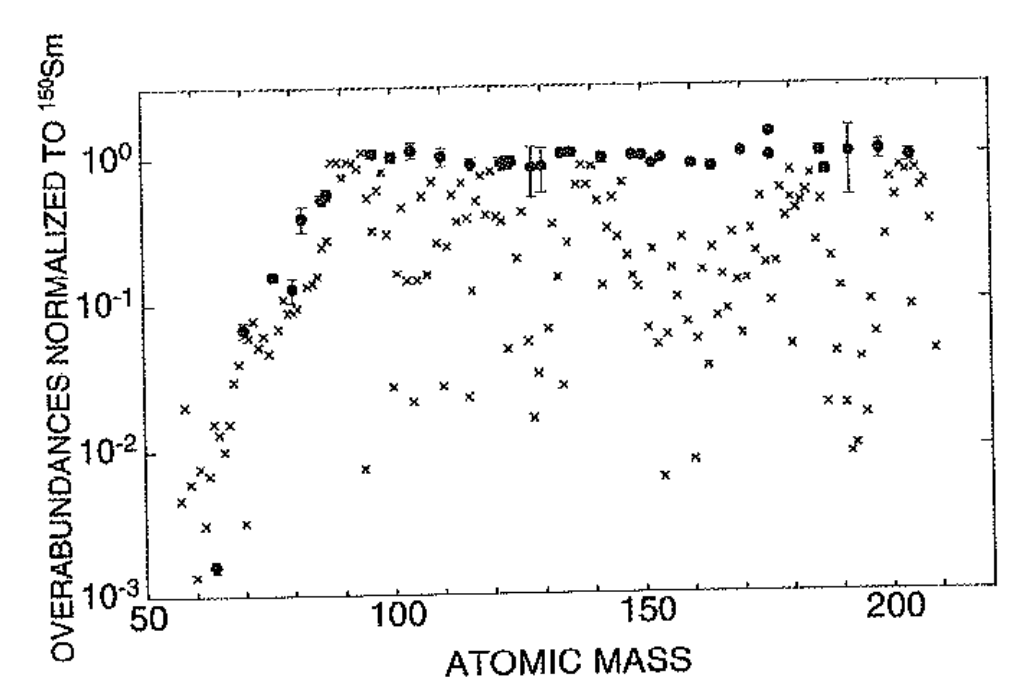
\includegraphics[width=\linewidth]{pdf/sproc.png}
\caption{\label{fig:sproc} Abundance distribution calculated in a
  simulation of a 1.5 \Msol\ star with metallicity Z$=0.01$.
  Abundances are shown as overabundance factors relative to the solar
  system abundances, with $^{150}$Sm used for scaling.  Circles
  represent s-process-only nuclei.  From~\cite{arlandinietal1999}.}
\end{figure}

Metal-poor AGB stars have fewer $^{56}$Fe seeds and thus each seed is
able to have a higher neutron exposure (\citealt{gallinoetal1998}).
Because of this higher nuclides can be synthesized and more nuclei can
accumulate in the termination loop of the s-process path.  Thus, lower
metallicity AGB stars provide a natural explanation for the strong
s-process component.  Specifically, \cite{travaglioetal2001} show that 
Pb production
in low- and intermediate-mass AGB stars reaches a maximum efficiency
at [Fe/H]$\sim 1$.  Metal poor AGB stars with enhanced Pb abundances
have been observed (\citealt{vaneck2001}; \citealt{vanecketal2003}).

The weak s-process component is thought to occur in core He burning in
massive stars
(e.g., \citealt{peters1968}; \citealt{couch1974}; \citealt{raiteri1991}).
\cite{iliadis2008} says more specifically it occurs in stars with mass
$\geq13$\Msol.  $^{14}$N left from the CNO cycle during H burning
(which piles up because proton capture on $^{14}$N is the rate
limiting step of the CNO cycle) fuses with two He nuclei to form
$^{22}$Ne which, as mentioned above, produces $^{25}$Mg and a neutron
when fused with a He nucleus.  This neutron source is activated for
$T \geq 0.25$ GK (\citealt{iliadis2008}); it is because of this high
temperature dependence that massive stars (which burn hotter) are the
major contributors to the weak s-process component.  

The scenarios described above (shell He and H burning in AGB stars and
core He burning in massive stars) are generally acknowledged to be the
most likely sites for the s-process; however, there are many other
sites which have been proposed and may contribute in some fraction to
overall s-process nuclide abundance.  The resolution of current
uncertainties in nuclear physics and stellar evolution, as well as new
discoveries made with the increasing fidelity of stellar evolution
simulations, may reveal these other proposed sites (or some new sites
altogether) to be significant players in the s-process story.

One such site proposed as contributing to the weak s-process 
is core carbon burning.  In this situation, He nuclei liberated by the
$^{12}$C$+^{12}$C reaction open up the $^{22}$Ne$+ \alpha \rightarrow
^{25}$Mg$+n$ neutron source using $^{22}$Ne left from core He
burning. There have been differing thoughts and results on the
significance of this site over the year, with a general trend in
recent years showing this site to be more significant than was
originally thought.  For example, \cite{arcoragi1991} concluded from their
simulation that core C burning was not more efficient than core
He burning at producing weak s-process nuclides and that He burning
causes the observed Galactic weak s-process abundances.  More recent
work has focused on the uncertainties of the core C burning rate and
their effects on stellar nucleosynthesis.  Specifically, \cite{bennettetal2012}
show that three different carbon burning models applied over a range
of stellar masses produce different
neutron exposures and, thus, s-process abundances.  Carbon burning
models with enhanced carbon burning rates produce lower temperatures
in the core, which
increases the efficiency of the $^{13}$C
neutron source as well as increase the lifetime of the carbon burning
stage, which both produce a higher neutron exposure.  They also show that very
high mass stars (M$\gtrsim25$\Msol) with a particular carbon-burning
model produce convective cores, which allows mixing of neutrons into
the center of the star and enhances neutron exposure.  This also
addresses another concern of s-process in core carbon burning, which
is that nuclei produced in carbon cores without convection are unable
to leave the core and thus are unable to leave the star as its
envelope is blown off via winds or supernovae and thus cannot
contribute to observed nuclide abundances.  However, based on the
s-process production of their most strongly enhanced carbon burning
rate they are able to rule that burning rate out because of an
over-production and over-mixing of those nuclides.  A moderately enhanced carbon
burning rate for masses $\gtrsim 20$\Msol\ is also similarly ruled
out.  Thus, limits on core carbon burning rates can be made based on
observed s-process abundances but the problem is still not completely
solved and core carbon burning may be a significant contributor to
observed s-process abundances.  \cite{bennettetal2012} also note in 
their paper the
existence of overlapping convective regions between the carbon core
and the carbon shell, which may also be a nucleosynthesis site worthy
of furture investigation. The models that produce overlapping
convective zones are the models that were ruled out by comparing
predicted s-process yields with observed solar system abundances; this
seems to indicate that that the models with overlapping convective
zones do not exist in nature and thus are not worth further
consideration.

%As noted above, convection can have a signficant role in observed 
%s-process abundances by pulling
%s-processed materials out of the depths of a star to regions where
%they can eventually become part of the interstellar medium (ISM)
%instead of remaining behind in the stellar remnant.  Convection also
%influences the s-process indirectly through its effects on stellar
%structure and temperature.  One aspect of 
%convection that has received a lot of attention is convection
%overshoot.  This is when
%material that is being convected 

Another controversy involved proton mixing with the main s-process
component that occurs in low mass AGB stars, as described previously.
Key to that process is the mixing of the intially separate $^{12}$C
and protons to allow the creation of $^{13}$C.  The $^{13}$C pocket is
thought to exist in a thin shell below the H envelope, requiring an
injection of H-rich material from the envelope above. There are
several proposed mechanisms for this proton injection.  One is
convective overshoot (\citealt{herwigetal1997}) where the momentum of
matter in convective motion carries it beyond the physical reach of
the convective zone and partly into the radiative zone, producing
mixing into the radiative zone. \cite{lugaroetal2003} use computer
simulations with prescription for convective overshoot to produce
s-process abundances consistent with many observations. However, they 
also show that the s-process abundances are more depedent on the
presence of a $^{13}$C pocket by manually putting $^{13}$C pockets
into simulations without convective overshoot and obtaining similar
results. Another proposed proton injection mechanism is rotationally
induced mixing.  \cite{langeretal1999} demonstrate that rotational
mixing in AGB stars can produce a $^{13}$C-rich layer although they
also point out that there is no evidence to suggest rotational mixing
over the convective overshoot of \cite{herwigetal1997} nor any reason
to believe that mechanisms cannot happen
simultaneously.  \cite{herwig2003} find that convective overshooting
has a greater positive effect on neutron exposure than does rotational
mixing but reach the conclusion that both effects are important for
obtaining observed s-process nuclide abundances since their convective
overshooting produces too large of a neutron exposure and their
rotational mixing tempers this large neutron
exposure.  \cite{siess2004} discuss the effect that rotational mixing
has on the formation of the neutron poison (a nuclide that absorbs
neutrons without participating in the s-process, thus reducing $N_n$)
$^{14}$N and how well it mixes with $^{13}$C; because of this, the
effect rotational mixing has on s-process efficiency is highly
dependent on the strength and duration of the shear mixing phase.  A
third proposed mixing mechanism is weak tubulence produced by gravity
waves.  \cite{denissenkov2003} show that it is possible that this mechanism may
produce a $^{13}$C pocket much wider than convective overshooting.

In conclusion, there are two main proposed sites for the s-process:
atmospheres of low-mass AGB stars and core He burning in massive
stars, corresponding to the main and weak s-process components,
respectively.  The strong s-process component, if it exists, can be a
result of the s-process proceeding in an environment with few seed
nuclei, allowing for a greater number of neutron captures on average
per seed nucleus.  A theoretical description of what happens at each
of these sites as well as simulations modeling nucleosynthesis at
these sites are fairly well developed and support the idea of
the s-process at these sites.  There is also some observation evidence
in support of these claims.  However, uncertainties in some nuclear
physics aspects of the neutron-creating and neutron poison reaction
chains as well as details of stellar evolution prevent definite
conclusions as to whether these sites are the sole significant
contributors to observed s-process abundances or if other sites also
provide significant contributions.  The resolution of these
uncertainties is closely tied to the progress of stellar evolution
models and simulations and so progress in this area will lead to
better understanding of s-process sites, as well as progress in
relevant areas of nuclear physics.  It is the author's opinion that
evidence in support of the main two proposed s-process sites is
sufficient to expect them as the main contributors to s-process
abundances but that other sites will be shown to also provide
significant contributions.


%Other stars in PUMO paper

%Neutron poison

Triple alpha.

LEPP?
%Third dredge up shutting off neutron capture?
